\documentclass[tikz,border=8pt]{standalone}
% Shared look for every TikZ diagram. Load with \input{../../tools/tikz-style.tex}
\usepackage[sfdefault]{roboto}
\usetikzlibrary{arrows.meta, positioning, shapes.geometric, calc, fit, backgrounds}
\definecolor{cblue}{HTML}{4C78A8}
\definecolor{corange}{HTML}{F58518}
\definecolor{cgreen}{HTML}{54A24B}
\definecolor{cred}{HTML}{E45756}
\definecolor{cpurple}{HTML}{B279A2}
\definecolor{cgrey}{HTML}{6B6B6B}
\tikzset{
  every picture/.style={font=\sffamily, line width=1.2pt},
  box/.style={draw=#1, fill=#1!12, rounded corners=4pt, align=center, inner sep=7pt, minimum height=1.1cm},
  box/.default=cgrey,
  arrow/.style={-{Stealth[length=3mm]}, draw=cgrey, line width=1.4pt},
  title/.style={font=\sffamily\bfseries\Large},
  note/.style={font=\sffamily\small, text=cgrey, align=center},
}
\AtBeginDocument{\hyphenpenalty=10000 \exhyphenpenalty=10000}

% The steering a circle needs (kinematic bicycle, Boyali et al. 2018 eq. 33; RO-070 2.2): the car turns about a point
% on its rear axle's line; the front wheel points square to the line from that point, so the angle at the centre is
% the steering angle and tan(delta) = L / R. Drawn 0.8 cm per metre: R = 10 m, L = 2.5 m, delta = 14.04 deg.
\begin{document}
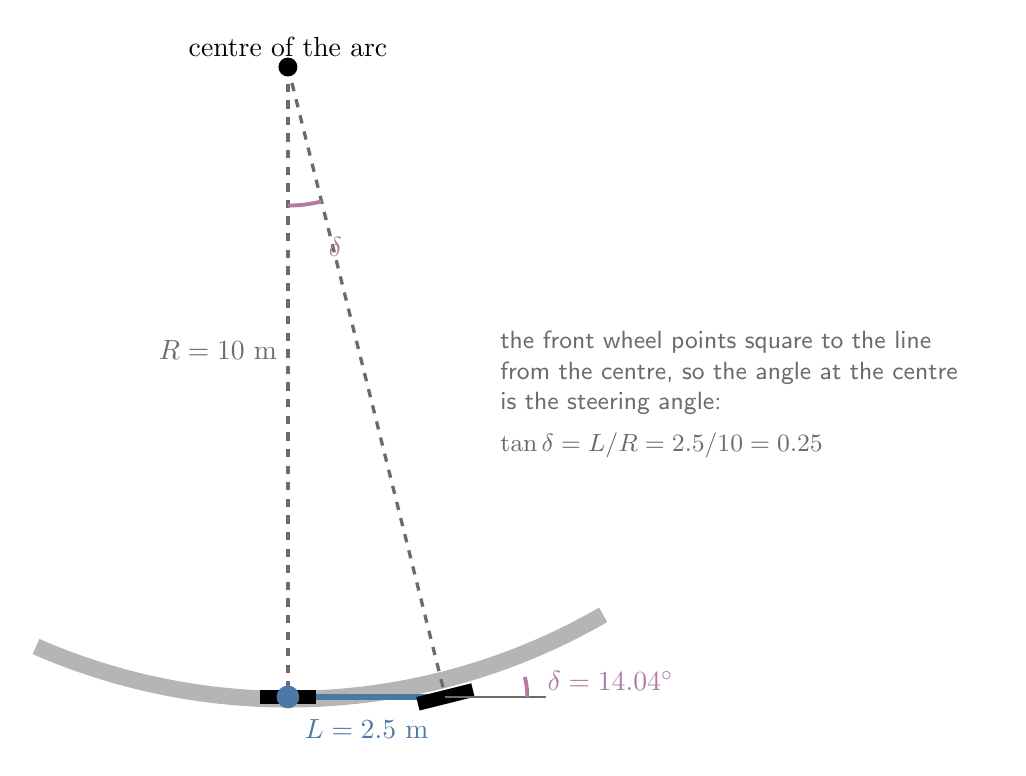
\begin{tikzpicture}[every node/.append style={font=\normalsize}, x=0.8cm, y=0.8cm]
  \coordinate (C) at (0,0);
  \coordinate (Rr) at (0,-10);
  \coordinate (F) at (2.5,-10);
  % the path circle
  \draw[cgrey!50, line width=6pt] (-4,-9.2) arc (246.4:300:10);
  % rear axle radius and front line to the centre
  \draw[cgrey, line width=1.2pt, dashed] (C) -- node[left, pos=0.45] {$R = 10$ m} (Rr);
  \draw[cgrey, line width=1.2pt, dashed] (C) -- (F);
  \draw[cpurple, line width=1.4pt] (0,-2.2) arc (270:284.04:2.2);
  \node[cpurple] at (0.75,-2.85) {$\delta$};
  % car body (bicycle): rear wheel, front wheel, axis
  \draw[cblue, line width=2pt] (Rr) -- node[below=4pt] {$L = 2.5$ m} (F);
  \draw[black, line width=5pt] (-0.45,-10) -- (0.45,-10);
  \draw[black, line width=5pt] ($(F)+(-0.4366,-0.1091)$) -- ($(F)+(0.4366,0.1091)$);
  \fill[cblue] (Rr) circle (0.18);
  % steering angle at the front wheel
  \draw[cgrey, line width=0.8pt] (F) -- ++(1.6,0);
  \draw[cpurple, line width=1.4pt] ($(F)+(1.3,0)$) arc (0:14.04:1.3);
  \node[cpurple, anchor=west] at ($(F)+(1.45,0.25)$) {$\delta = 14.04^\circ$};
  \fill[black] (C) circle (0.15);
  \node[anchor=south] at (C) {centre of the arc};
  \node[note, anchor=west, text width=6.2cm, align=left] at (3.2,-5.2) {the front wheel points square to the line from the centre, so the angle at the centre is the steering angle:\\[4pt] $\tan\delta = L / R = 2.5 / 10 = 0.25$};
\end{tikzpicture}
\end{document}
